\chapter{Licencias de software}
%\chapterauthor{
%Bartoszensky, Luciano
%,
%Cuello, Nahuel Ignacio
%,
%Ferrero, Facundo
%,
%Niño, Jeremías
%,
%Segurado, Lucas Martín
%,
%Zamora, Fernando
%}


%\section{¿Qué es una Licencia de Software Libre?}
\mysection{¿Qué es una licencia de software?}{¿Qué es una licencia?}

Una licencia de software es un documento (generalmente en formato digital) a través del cual la empresa desarrolladora o dueña del software otorga al receptor o usuario ciertos derechos sobre el software desarrollado. 

En general todo software, independientemente de su forma de distribución, ya sea como pieza separada de software o como servicio (a través de Internet), tiene una licencia (también conocida como EULA por las siglas en inglés de \emph{End-User License Agreement} o Acuerdo de Licencia con el Usuario Final) o un documento de ``condiciones de uso''. 

De lo anterior debe quedar claro que el software generalmente no se vende (ni su código fuente, ni su código binario) sino que se comercializa su derecho a usarlo por un tiempo determinado o a eternidad. Este concepto es importante, porque es la base del modelo de negocios mayoritario en la industria del software, tal como veremos en un capítulo posterior. 

Si la licencia o EULA otorga al usuario las 4 libertades de la definición de software libre (ver capítulo 1) se dice que es una ``licencia libre''. Si la licencia es compatible con las 10 cláusulas que definen al software de fuentes abiertas (según la definición de la OSI que dimos en el capítulo 1) se dice que es una  ``licencia de software de fuentes abiertas''. En caso contrario será una ``licencia no libre'' o, como muchas veces se las menciona, una ``licencia privativa'' (porque se priva al usuario de esas libertades o derechos).

A su vez, las licencias libres se clasifican en los siguientes dos tipos, según si permiten al usuario modificar la licencia para la redistribución del software.

\begin{itemize}
\item Permisivas: son las licencias libres que permiten al usuario redistribuir el software con otra licencia diferente, ya sea libre o privativa. Las licencias MIT, BSD y Apache son ejemplos de este tipo de licencias.

%\item Copyleft débil: hace referencia a las licencias que no se heredan a todos los trabajos derivados, dependiendo a menudo de la manera en que estos se hayan derivado. Se utiliza generalmente para la creación de bibliotecas de software, con el fin de permitir que otros programas puedan enlazar con ellas y ser redistribuidos, sin el requerimiento legal de tener que hacerlo bajo la nueva licencia copyleft. Solamente se requiere distribuir los cambios sobre el software con copyleft débil, no los cambios sobre el software que enlaza con el. Un claro ejemplo de este tipo de licencias es la Licencia Pública de Mozilla.

\item Robustas: obliga al usuario a utilizar la misma licencia para la redistribución del software libre. Esto asegura (u obliga) a que el software desarrollado como libre siempre se mantenga libre, independientemente de quién lo modifica y redistribuye posteriormente. El ejemplo más conocido de este tipo de licencia es la familia de licencias GPL (\emph{GNU General Public License}).
\end{itemize}

%\section {Copyleft, Copyright y Creative Commons}
\mysection{Conceptos legales (y no tanto)}{Conceptos legales}

Para la ley argentina el software es una obra protegida por la propiedad intelectual. La ley original era la 11.723, que fue promulgada en 1933 y luego modificada para adaptarse a los tiempos. En 1998 se promulgó la ley 25.036, que modifica a la anterior y establece en su artículo primero\footnote{El texto actual de la ley 11.723, modificado por la ley 25.036 y otros decretos, está disponible en \url{http://servicios.infoleg.gob.ar/infolegInternet/anexos/40000-44999/42755/texact.htm}} que ``las obras científicas, literarias y artísticas comprenden los escritos de toda naturaleza y extensión, {\bf entre ellos los programas de computación fuente y objeto}''. 

En general la ley reconoce al/la autor/a de la obra (en nuestro caso los/as desarrolladores/as del software) y a los/as titulares del derecho de propiedad intelectual. La autoría es un derecho moral y es eterno, es decir, nunca se puede cambiar quién es el o la autora de una obra, independientemente de quién tenga el derecho a la propiedad. En cambio el derecho a la propiedad, o también llamado ``derecho a copia'' o \emph{copyright} en inglés, es un derecho patrimonial (el poseedor de este derecho puede pedir resarcimiento económico por el uso de su obra) y tiene limitaciones temporales que dependen del tipo de obra y la legislación de cada país.

El artículo 4 inciso (d) de la nueva ley de propiedad intelectual argentina establece que ``las personas físicas o jurídicas cuyos dependientes contratados para elaborar un programa de computación hubiesen producido un programa de computación en el desempeño de sus funciones laborales, salvo estipulación en contrario'' son titulares del derecho a la propiedad intelectual del software. Los/as desarrolladores/as contratados retienen el derecho moral de autoría del software, pero quien tiene el derecho patrimonial para obtener rédito económico de dicho software es la empresa que los contrató.

A partir del término inglés \emph{copyright}, que establece al dueño de los derechos sobre una obra, Richard Stallman propuso, como otro juego de palabras, el concepto de \emph{copyleft} para indicar que el autor de la obra otorga los derechos de dicha obra a los usuarios\footnote{En inglés \emph{right} significa tanto ``derecho'' en el sentido legal como ``derecha'' en ideología política, mientras que \emph{left} significa tanto ``izquierda'' en el sentido político como ``dejar'' o ``ceder'' en el sentido de ceder derechos.}. En ese caso, las licencias libres serían consideradas como \emph{copyleft}, ya que otorgan los derechos de uso, modificación y distribución a los usuarios, mientras que las licencias privativas serían \emph{copyright}, pues los propietarios retienen la mayoría de esos derechos.

Recientemente aparecieron conceptos derivados, tales como \emph{copyfarleft} y \emph{copyfair}, que establecen ciertas reglas más estrictas para evitar que empresas que no colaboraron en el desarrollo de la obra puedan lucrar con su uso. En el caso de \emph{copyfarleft} solo empresas de propiedad de sus trabajadores (por ejemplo, cooperativas) pueden beneficiarse económicamente de la obra. Por su parte, usar \emph{copyfair} exige a las empresas que no colaboraron en el desarrollo el pago de una tasa si quieren beneficiarse económicamente del producto. Un ejemplo de este tipo de licencia es la PPL (\emph{Peer Production License})\footnote{PPL (Peer Production License): \url{https://wiki.p2pfoundation.net/Peer_Production_License}}.
\\


\section{Compatibilidad de licencias}
%\mysection{Compatibilidad de licencias}{Compatibilidad de licencias}

Es fácil pensar en un programa informático y su correspondiente licencia. Sin embargo, sabemos que actualmente los programas se constuyen por medio de la combinación de diferentes paquetes de software, librerías\footnote{Entendemos que el término ``librería'' para referirse a una colección de funciones de software es una mala traducción del término en inglés \emph{library}. Pero dado lo común de su uso, lo adoptamos en este texto.}, módulos nuevos y viejos, modificados o no. Cada parte de un programa, al provenir de diferentes fuentes, puede tener diferentes licencias, por lo cual es importante entender bajo qué términos se puede licenciar el software desarrollado de esta forma. 

Las licencias pueden tener cláusulas contradictorias entre sí, que hacen imposible combinar el código para crear nuevos paquetes de software. Por ejemplo si una licencia de un paquete de software dice que las versiones modificadas deben mencionar a todos los/as desarrolladores/as y la licencia de otro paquete dice que las versiones modificadas no pueden contener atribución de autoría adicional, entonces crear un software que utilice ambos paquetes modificados es posible técnicamente pero no se puede asociar una licencia que satisfaga a ambas licencias originales. 

Si bien este problema no es exclusivo del software libre, existen más trabajos para simplificar el análisis de la incompatibilidad o compatibilidad de licencias en este tipo de software que en el privativo. Un ejemplo de tablas de compatilibidad de licencias de software libre y de fuentes abiertas son las matrices realizadas por la Oficina de Coordinación de Software Libre de \emph{Xunta de Galicia}\footnote{Matriz de compatibilidad de licencias de software libre: \url{https://www.mancomun.gal/es/documento/matriz-de-compatibilidad-de-licencias-de-software-libre/}}, que mostramos en la Figura~\ref{figMatriz}. Para entender la diferencia entre las dos matrices se debe tener en cuenta que un componente de software es ``estático'' cuando se combina con el resto del paquete en tiempo de compilación, copiándose dentro del ejecutable o binario de la aplicación, y es ``dinámico'' cuando es invocado en tiempo de ejecución, sin ser parte del código binario de la aplicación.

\begin{figure}[h!]
\centering
\begin{subfigure}{\linewidth}
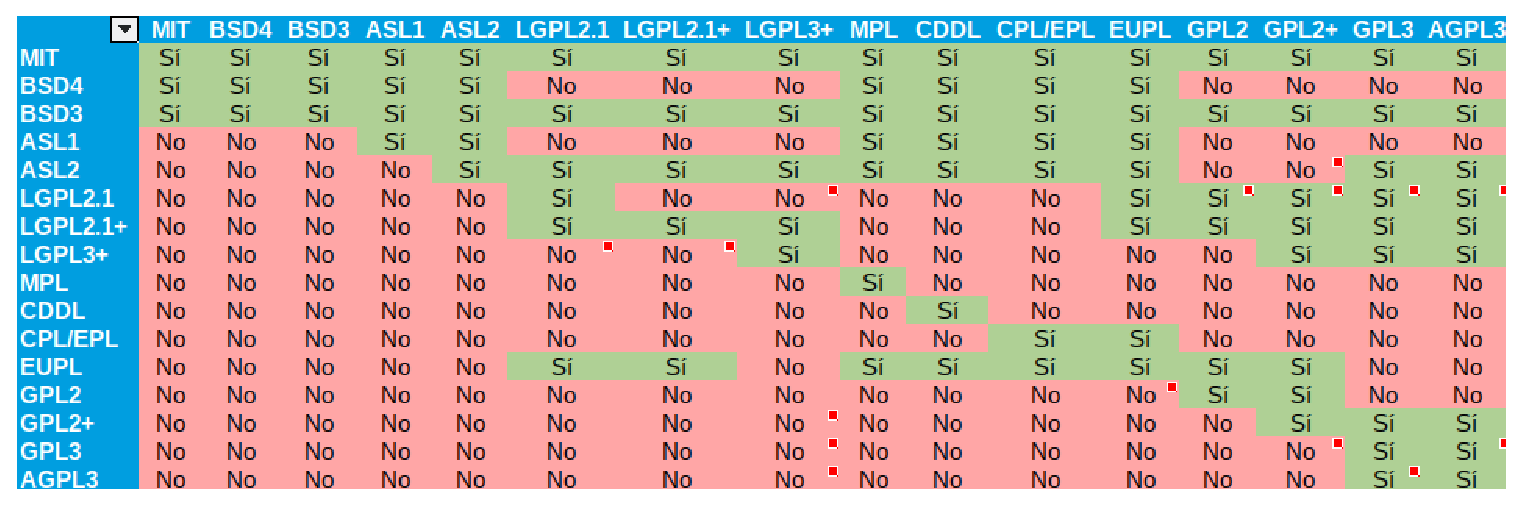
\includegraphics[scale=.5]{imagenes/matriz-estatica.eps}
\caption{Matriz de compatibilidad de licencias de paquetes de software estáticos.}
\end{subfigure}
\begin{subfigure}{\linewidth}
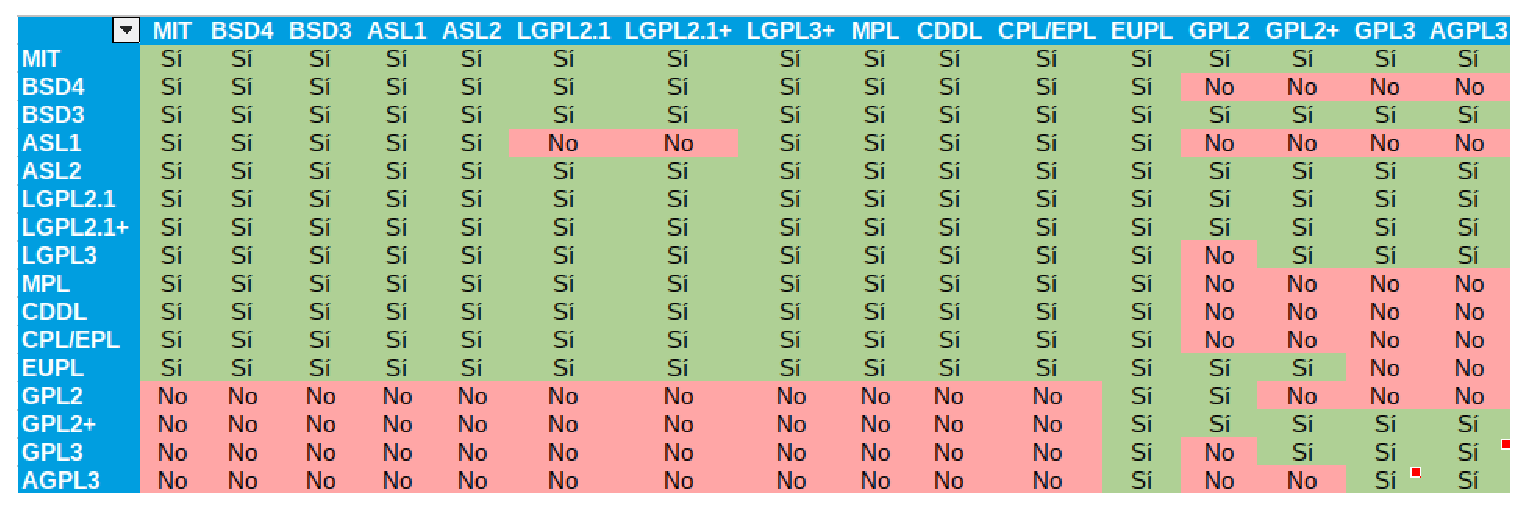
\includegraphics[scale=.5]{imagenes/matriz-dinamica.eps}
\caption{Matriz de compatibilidad de licencias de paquetes de software dinámicos.}
\end{subfigure}
\caption{Matrices de compatibilidad realizadas por el Centro Nacional de Referencia de Aplicación de las Tecnologías de la Información y Comunicación (CENATIC) en 2019}
\label{figMatriz}
\end{figure}

%\begin{itemize}
%\item {\bf Copyleft}
%Estrategia legal la cual permite hacer que el código sea libre, es decir, que pueda ser utilizado por cualquiera, modificarlo y mejorarlo para cualquier propósito, distribuir versiones originales y mejoradas con o sin lucro sin pedir permiso a nadie. Toda nueva versión o copia está basada en las mismas condiciones que el original.
%\item {\bf Copyright}
%Licencia más restrictiva, sólo el autor puede utilizarlo y si alguien quiere usarlo debe pedirle permiso al autor y pagarle. Si el software no tiene definida ningún tipo de licencia, adopta por defecto la copyright, cabe aclarar que su registro no es obligatorio. 
%\item {\bf Creative Commons}
%Determina cómo va a circular el software en internet, es decir, algunos autores pueden dar derechos a otras personas, son gratuitas y su registro no es obligatorio.
%\end{itemize}


%La característica peculiar de estas licencias se debe a que no poseen copyleft, ya que el trabajo derivado no tiene por qué mantenerse con el mismo régimen de derechos de autor que el original. Esto maximiza la libertad para quien recibe el software y quiere desarrollar algo derivado, permitiéndole elegir entre el amplio abanico de licencias existentes. No obstante, desde el punto de vista de los usuarios, esto se puede considerar como una restricción a su libertad, en el sentido de que el software propietario siempre restringe las libertades de los usuarios del mismo y las licencias permisivas, abren esta posibilidad. Los ejemplos más conocidos de este tipo de licencias son la Licencia MIT y la Licencia BSD.

%\section{Organismos}
%\begin{itemize}
%\item {\bf Fundación para el software libre(FSF) }
%Creada por Richard Stallman en 1985 con la finalidad de eliminar restricciones sobre copias, redistribución, entendimiento y modificación .Esto ayudó a promover el software libre, especialmente en el desarrollo de SO GNU. Actualmente se centra en asuntos legales, organizativos y promocionales del software libre. Stallman fue el creador del Copyleft 
%
%\item {\bf Open Source Initiative(OSI)}
%Creada por Bruce Perens y Eric S. Raymond en 1998 con la finalidad de promover el software libre. A fines del 1998 publicaron el código fuente de Netscape Communicator dadas las pérdidas y dura competencia con Internet Explorer de Windows. No podían competir ya que IE venía gratis con Windows, en cambio su producto era por separado y pago. Luego con la publicación del código fuente, hubo un grupo de personas que introdujo el término mercadotecnia que permitió levantar al software libre debido a que era más amigable. Gracias a este proyecto, surgen otros como Mozilla. 
%
%\item {\bf Proyecto Fedora}
%Comunidad responsable de la distribución de Fedora y otros proyectos. Es la fusión de Red Hat y el antiguo proyecto Fedora en 2003. El viejo Fedora desarrollaba paquetes para las viejas distribuciones de Red Hat (RHL 8 Y 9, FC1 Y 2).
%
%\item {\bf Directrices de software libre de Debian}
%Directrices que permiten ver si una licencia de software es una licencia de software libre y además si alguna licencia y software pueden incluirse en la distribución de Debian. Algunas de las directrices que podemos mencionar son:
%
%\begin{itemize}
%	\item Libre redistribución
%	\item Inclusión del código fuente
%	\item Permitir que las modificaciones y trabajos derivados sean hechos bajo la misma licencia
%	\item	Integridad del código fuente del autor, se debe permitir cuando menos la distribución de modificaciones por medio de parches
%	\item Sin discriminación de personas o grupos
%	\item Sin discriminación de áreas de iniciativa, como el uso comercial
%	\item Distribución de la licencia, se necesita aplicar a todo al que se redistribuya el programa
%	\item La licencia no debe ser específica a Debian, básicamente reiteración del punto anterior
%	\item La licencia no debe contaminar otro software
%\end{itemize}
%\end{itemize}
%%\newpage




%\section {Tipos de Licencias}
%El software no se vende, se licencia. Una licencia es aquella autorización formal con carácter contractual que un autor de un software da a un interesado para ejercer actos de explotación legales. Es decir, el software no se compra, sino que se adquieren una serie de derechos sobre el uso que se le puede dar. En las licencias de software libre esos derechos son muy abiertos y permisivos, apenas hay restricciones al uso de los programas. De ahí que ayude al desarrollo de la cultura. Pueden existir tantas licencias como acuerdos concretos se den entre el autor y el licenciatario. Desde el punto de vista del software libre, existen distintas variantes del concepto o grupos de licencias, las mismas pueden clasificarse en distintos grupos:\\


%\section{Papel de la FSF y OSI}
%
%{\bf Licencias de código abierto aprobadas por el OSI}
%El grupo OSI define y mantiene una lista de licencias de código abierto aprobadas por el mismo. OSI está de acuerdo con la FSF en la mayoría de las licencias de software libre, pero difiere en algunos de la lista de la FSF. Por ejemplo, se posiciona del lado de la definición de código abierto más que de la definición de software libre. Considera que las leyes del grupo licencias de software libre permisivas son una referencia de implementación de una licencia software libre. Esto es sus requerimientos para aprobar las licencias son diferentes.
%\\
%{\bf Licencias de software libre aprobadas por la FSF}
%La FSF, el grupo que mantiene la definición de software libre, mantiene una lista de licencias de software libre no exhaustiva.12 La FSF es una organización sin ánimo de lucro cuya misión es promover la libertad de los usuarios de los ordenadores y defender los derechos de todos los usuarios del software libre. Los desarrolladores de software libre garantizan que todo el mundo tenga los mismos derechos para sus programas, cualquier usuario puede estudiar el código fuente, modificarlo, y compartir el programa. Por el contrario, la mayoría del software lleva una nota que impide a los usuarios estos derechos básicos, dejando a los usuarios susceptibles a los deseos de sus propietarios y a la vulnerabilidad de ser vigilados. La FSF prefiere las licencias de software libre copyleft (share-alike) mejor que las licencias de software libre permisivas para la mayoría de los propósitos. En su lista distingue entre las licencias de software libre que son compatibles o incompatibles con el la GPL de copyleft de la FSF.
%
%%\newpage

%\section{Garantìas, condiciones y limitaciones brindadas por las licencias}
%\begin{itemize}
%\item Garantìas: Son aquellas características del software que son permitidas o autorizadas por la licencia.
%\begin{itemize}
%\item Usar: Se garantiza el uso del software
%\item Distribuir/Comerciar: Se permite su distribución y/o comercialización.
%\item Modificar: Se permite modificar características y funcionalidades del programa.
%\item Mejorar el programa y publicar las mejoras: Se pueden sugerir cambios y permitir que dichos cambios se lleven a cabo.
%\item Derechos de patente para sus contribuidores: Las patentes dependen de las leyes nacionales respecto a las licencias del software.
%\end{itemize}
%\item Condiciones: Son aquellas características que debe poseer todo software que derive del poseedor de la licencia
%\begin{itemize}
%\item Misma licencia: Debe mantener su licencia cuando se realicen modificaciones.
%\item Revelar fuente: Código fuente debe estar disponible cuando se distribuya el software
%\item Informar de licencia y copyright: Se debe poseer una licencia e informar del copyright junto con el software
%\item Red como medio de distribución: Se debe poder utilizar la red para recibir una copia del código fuente
%\item Cambios documentados
%\end{itemize}
%\item Limitaciones: Son todas las características que no garantiza la licencia respecto al uso del software.
%\begin{itemize}
%\item Responsabilidad: No se hacen responsables por el uso dado al software
%\item Garantía: No se provee ninguna garantía
%\item Uso de marca registrada: No garantiza el uso de la marca registrada
%\end{itemize}
%\end{itemize}

